\begin{frame}[c]
\begin{center}
\Huge Adversarial training
\end{center}
\end{frame}

\begin{frame}{Approach 1}
    \begin{block}{Run 1}
\begin{itemize}
    \item Same hyper-parameters for both networks
    \item Adversary uses only 3 layers
\end{itemize}
    \end{block}
    \begin{block}{Setup}
    \begin{itemize}
    \item Input: \num{14} variables motivated by a BDT variable scan.
    \item Hidden layers: \num{6}(\num{3}) \ELU layers $\times$ \num{128} nodes each
    \item Output layer: \num{1} \SIGMOID node
    \item Optimisation: SGD, Learning rate $=0.06$, momentum $=0.3$, no nesterov, no decay
    \item Duration: 400 iteration
    \item $\lambda = 10$
    \end{itemize}
    \end{block}
\end{frame}

\begin{frame}{Approach 1 - Run 1 - Results}
    \begin{figure}[htbp]
    \centering
    \begin{subfigure}[b]{0.47\textwidth}
        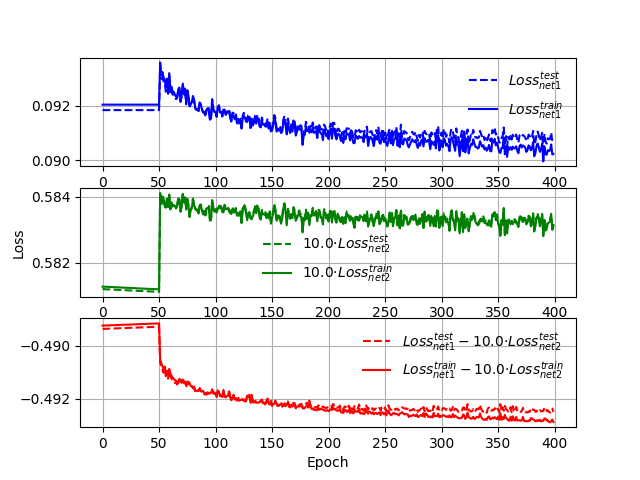
\includegraphics[width=\textwidth]{app1/full_classic_losses.png}
        %\caption{}
        \label{fig:simple:final:sepa}
    \end{subfigure}
\quad
    \begin{subfigure}[b]{0.47\textwidth}
        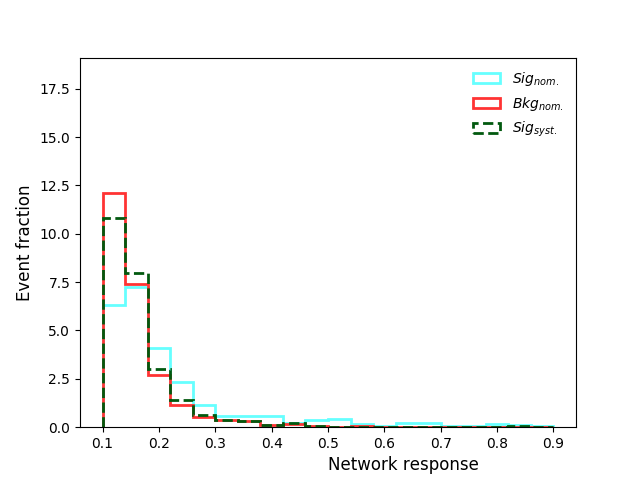
\includegraphics[width=\textwidth]{app1/full_classic_syst.png}
        %\caption{}
        \label{fig:simple:final:syst}
    \end{subfigure}
    \end{figure}
    \begin{itemize}
        \item Both losses decreasing
        \item Only combined losses depend on $\lambda$
        \item Bad separation
        \item High sensitivity to systematics
    \end{itemize}
\end{frame}

\begin{frame}{Approach 1}
\begin{block}{Setup of the adversary}
    \begin{itemize}
    \item Input: \num{14} variables motivated by a BDT variable scan.
    \item Hidden layers: \num{3} \ELU layers $\times$ \num{32} nodes each
    \item Output layer: \num{1} \SIGMOID node
    \item Optimisation: SGD, Learning rate $=0.001$, momentum $=0.$, no nesterov, no decay
    \item Duration: 400 iteration
    \item $\lambda = 0.1$
    \end{itemize}
    \end{block}
\end{frame}

\begin{frame}{Approach 1 - Run 2 - Results}
    \begin{figure}[htbp]
    \centering
    \begin{subfigure}[b]{0.47\textwidth}
        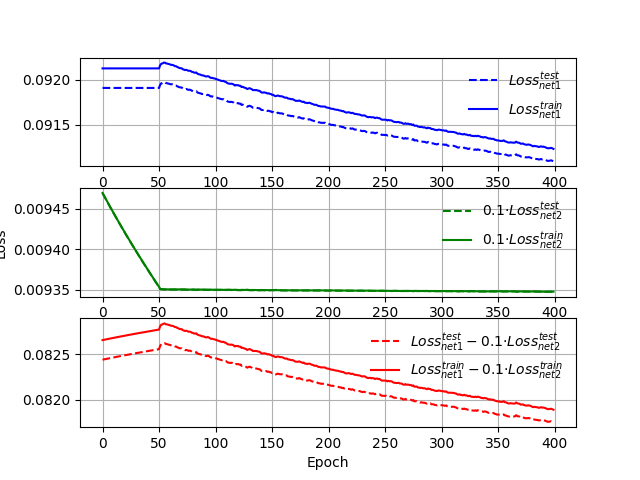
\includegraphics[width=\textwidth]{app1/half_classic_losses.png}
        %\caption{}
        \label{fig:simple:final:sepa}
    \end{subfigure}
\quad
    \begin{subfigure}[b]{0.47\textwidth}
        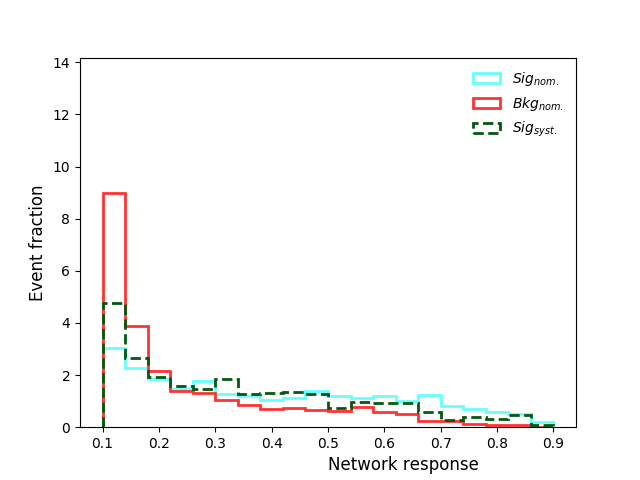
\includegraphics[width=\textwidth]{app1/half_classic_syst.png}
        %\caption{}
        \label{fig:simple:final:syst}
    \end{subfigure}
    \end{figure}
    \begin{itemize}
        \item Visible separation
        \item Adversary loss stops falling
        \item No improvement in the sensitivity visible
    \end{itemize}
\end{frame}

\begin{frame}{Approach 2}
\begin{figure}
    \centering
    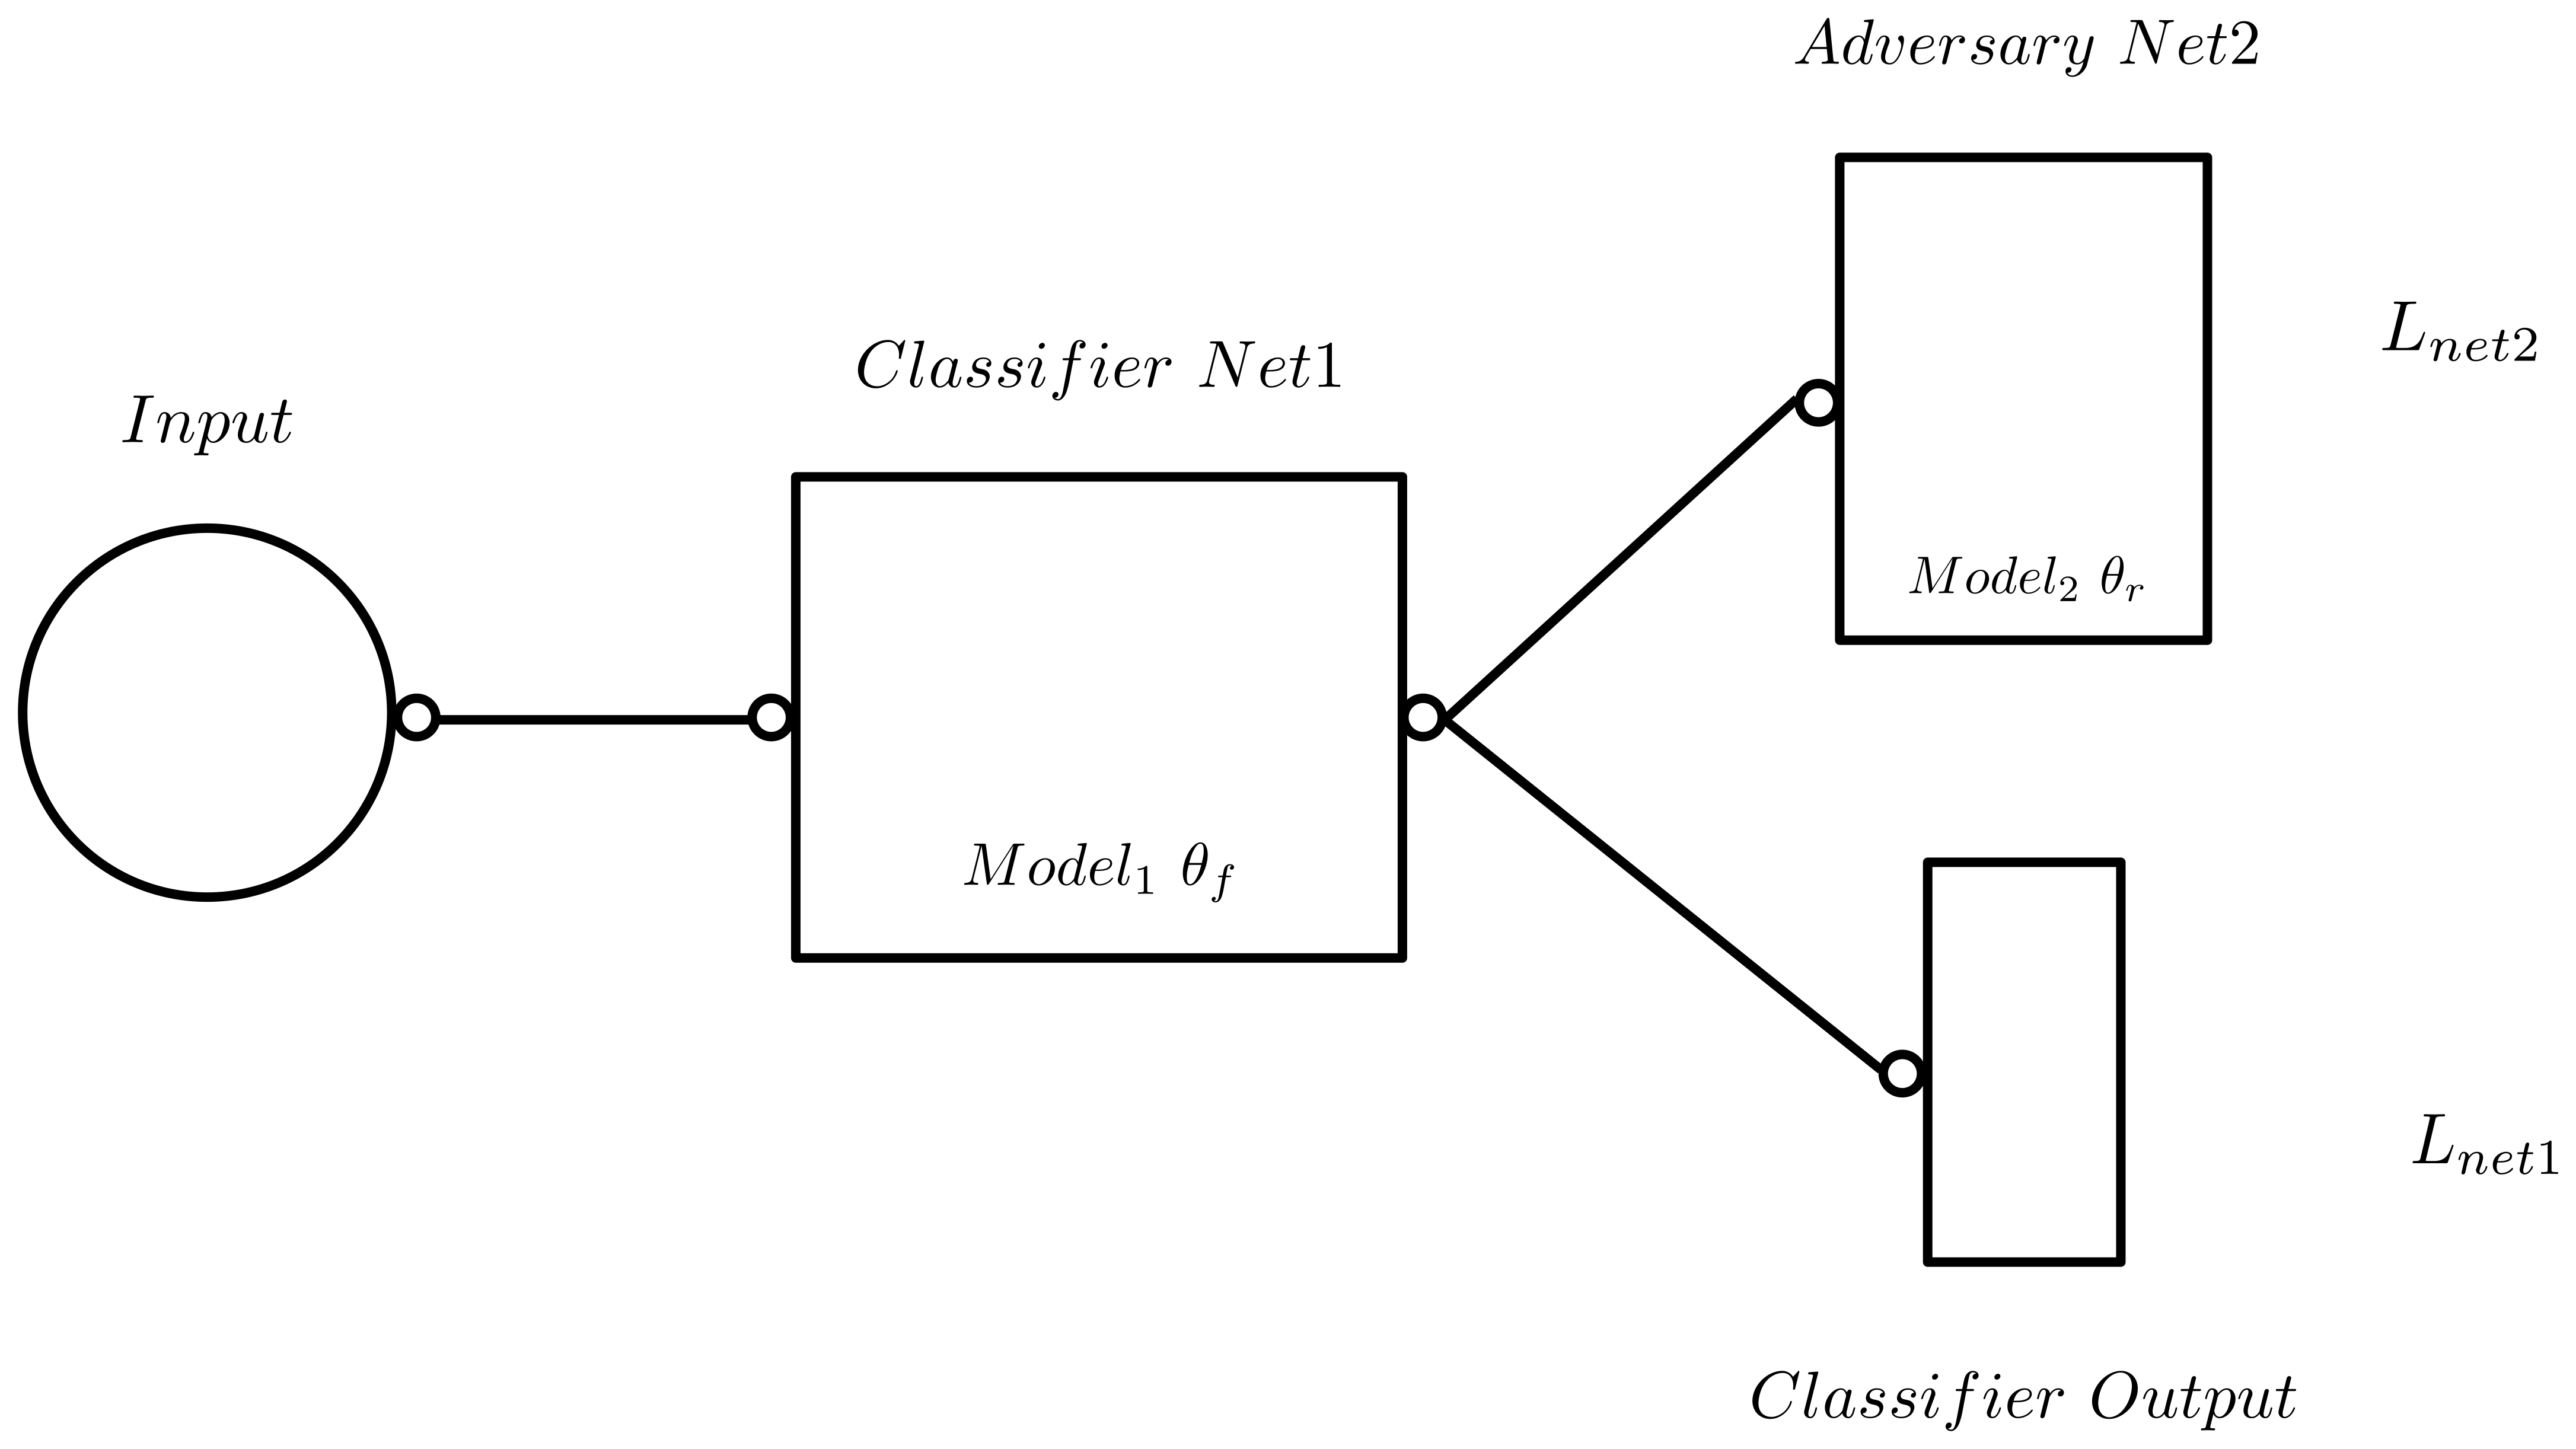
\includegraphics[width=0.8\textwidth]{figures_theory/ANN_sketch.png}
    %\caption{Caption}
\end{figure}
    \begin{block}{Input the last hidden layer to the adversary}
        \begin{itemize}
            \item More information provided
            \item Possible danger: Missing last decision step
        \end{itemize}
    \end{block}
\end{frame}


\begin{frame}{Approach 2 Results}
    \begin{figure}[htbp]
    \centering
    \begin{subfigure}[b]{0.47\textwidth}
        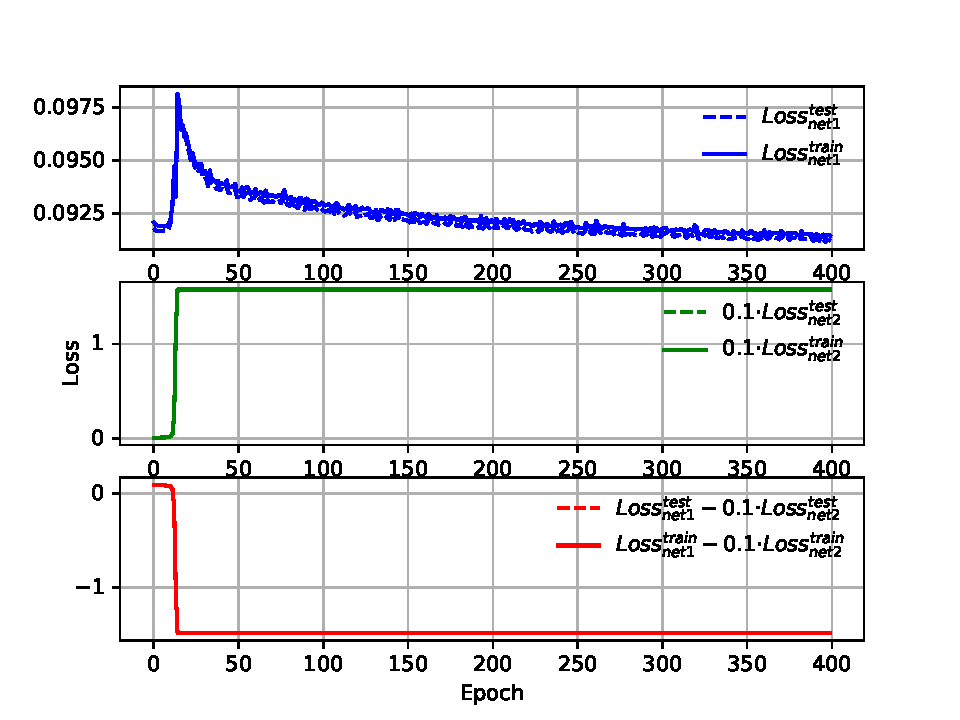
\includegraphics[width=\textwidth]{app2/app2_losses2.pdf}
        %\caption{}
        \label{fig:simple:final:sepa}
    \end{subfigure}
\quad
    \begin{subfigure}[b]{0.47\textwidth}
        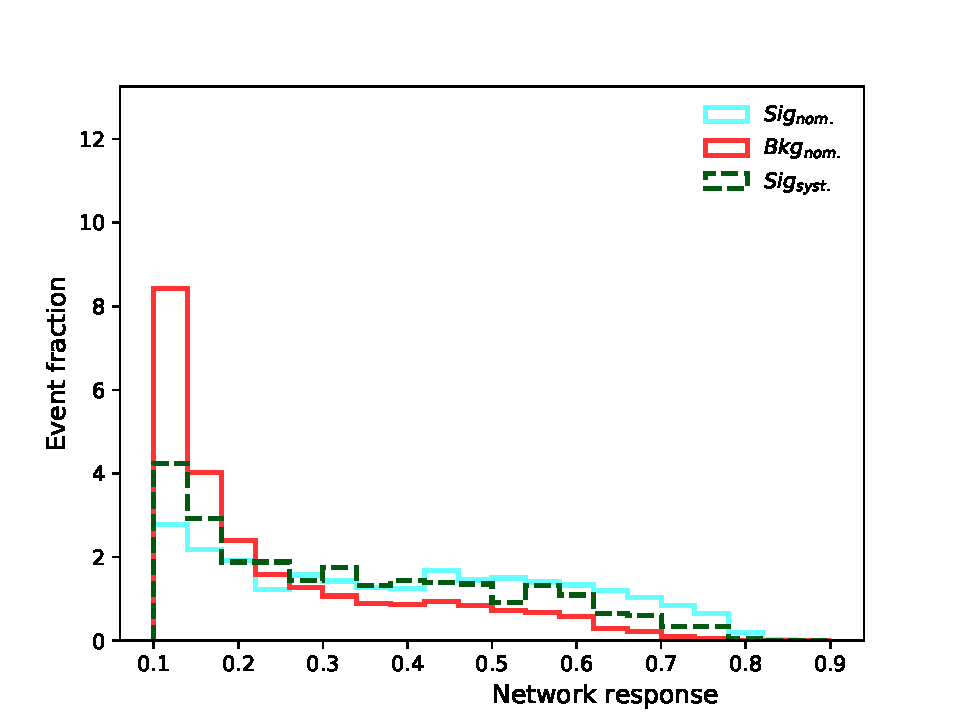
\includegraphics[width=\textwidth]{app2/app2_syst.pdf}
        %\caption{}
        \label{fig:simple:final:syst}
    \end{subfigure}
    \end{figure}
        \begin{itemize}
            \item Losses behave as desired
            \item steep rise, although partially due to scale
            \item $\lambda$ almost unusable due to difference in magnitude
            \item still high sensitivity
        \end{itemize}
\end{frame}

\begin{frame}{Approach 3}
\begin{block}{Assumption}
    Dimension of the hidden layer is too high
\end{block}
\begin{block}{Easy workaround}
    \begin{itemize}
        \item Add an intermediate layer
        \item Reduced to 16 nodes
    \end{itemize}
\end{block}
\end{frame}

\begin{frame}{Approach 3 Results}
    \begin{figure}[htbp]
    \centering
    \begin{subfigure}[b]{0.47\textwidth}
        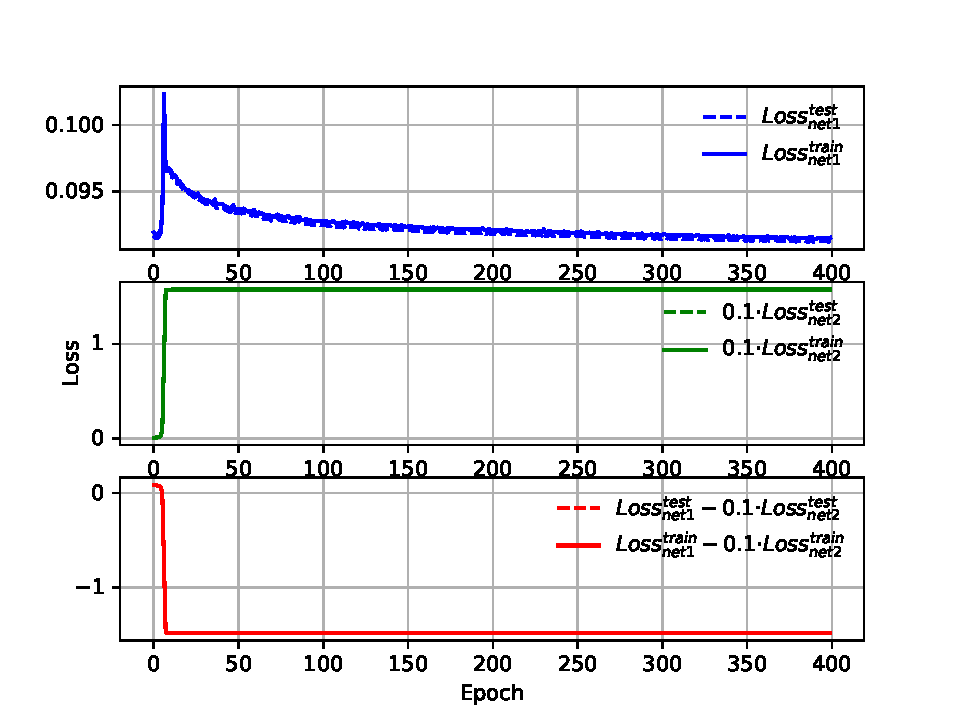
\includegraphics[width=\textwidth]{app3/app3_losses2.pdf}
        %\caption{}
        \label{fig:simple:final:sepa}
    \end{subfigure}
\quad
    \begin{subfigure}[b]{0.47\textwidth}
        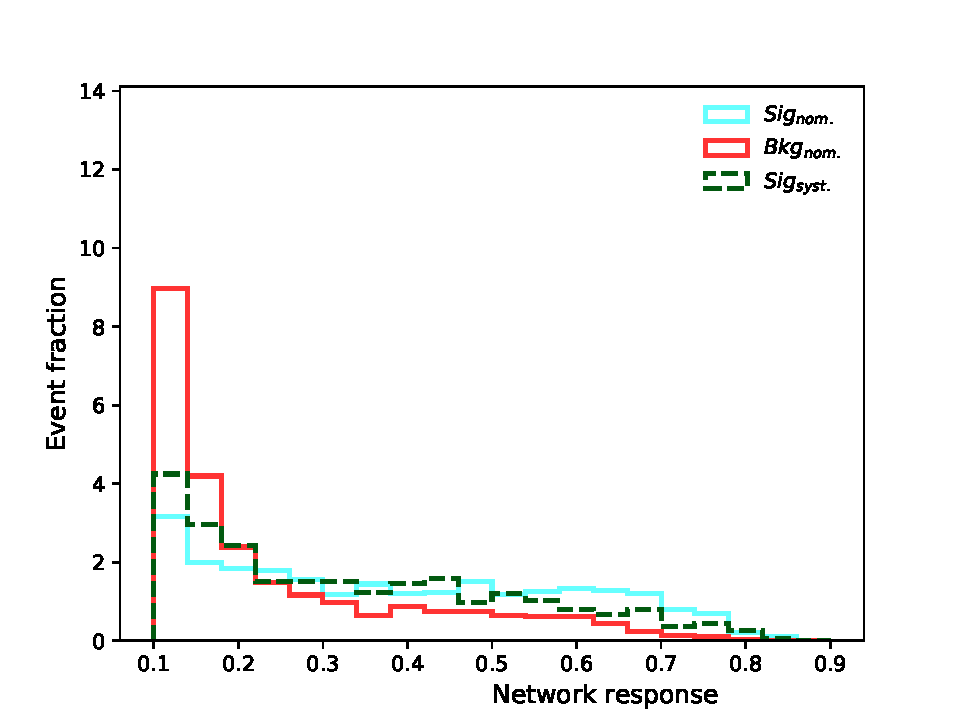
\includegraphics[width=\textwidth]{app3/app3_syst.pdf}
        %\caption{}
        \label{fig:simple:final:syst}
    \end{subfigure}
    \end{figure}
        \begin{itemize}
            \item Almost no difference
            \item Slightly higher stability
        \end{itemize}
\end{frame}
